\documentclass{article}
\usepackage[utf8]{inputenc}
\usepackage{amstext}
\usepackage{amsmath}
\usepackage{amsfonts}
\usepackage{graphicx}
\usepackage[margin=1in, paperwidth=8.5in, paperheight=11in]{geometry}
\usepackage{gensymb}
\usepackage{indentfirst}
\usepackage{textcomp}
\usepackage{upgreek }
\usepackage{siunitx}
\usepackage{enumitem}

\usepackage[american]{circuitikz}

\title{Circuits Postlab 7}
\author{Byron Wasti}
\date{April 2017}

\begin{document}
\maketitle

The $p$MOS and $n$MOS circuits behave in very similar ways, except that their respective current characteristics are flipped along the y-axis. The voltage characteristic is inverted as well for the $p$MOS circuit, on both the x-axis and y-axis.

Both of these differences make sense, since the $p$MOS and $n$MOS transistors are essentially opposites of each other.

\begin{figure}[h]
    \centering
    \includegraphics[width=\textwidth]{../12plot}
    \caption{Current and Voltage characteristic of pMOS Circuit}
    \label{fig:two}
\end{figure}

\begin{figure}[h]
    \centering
    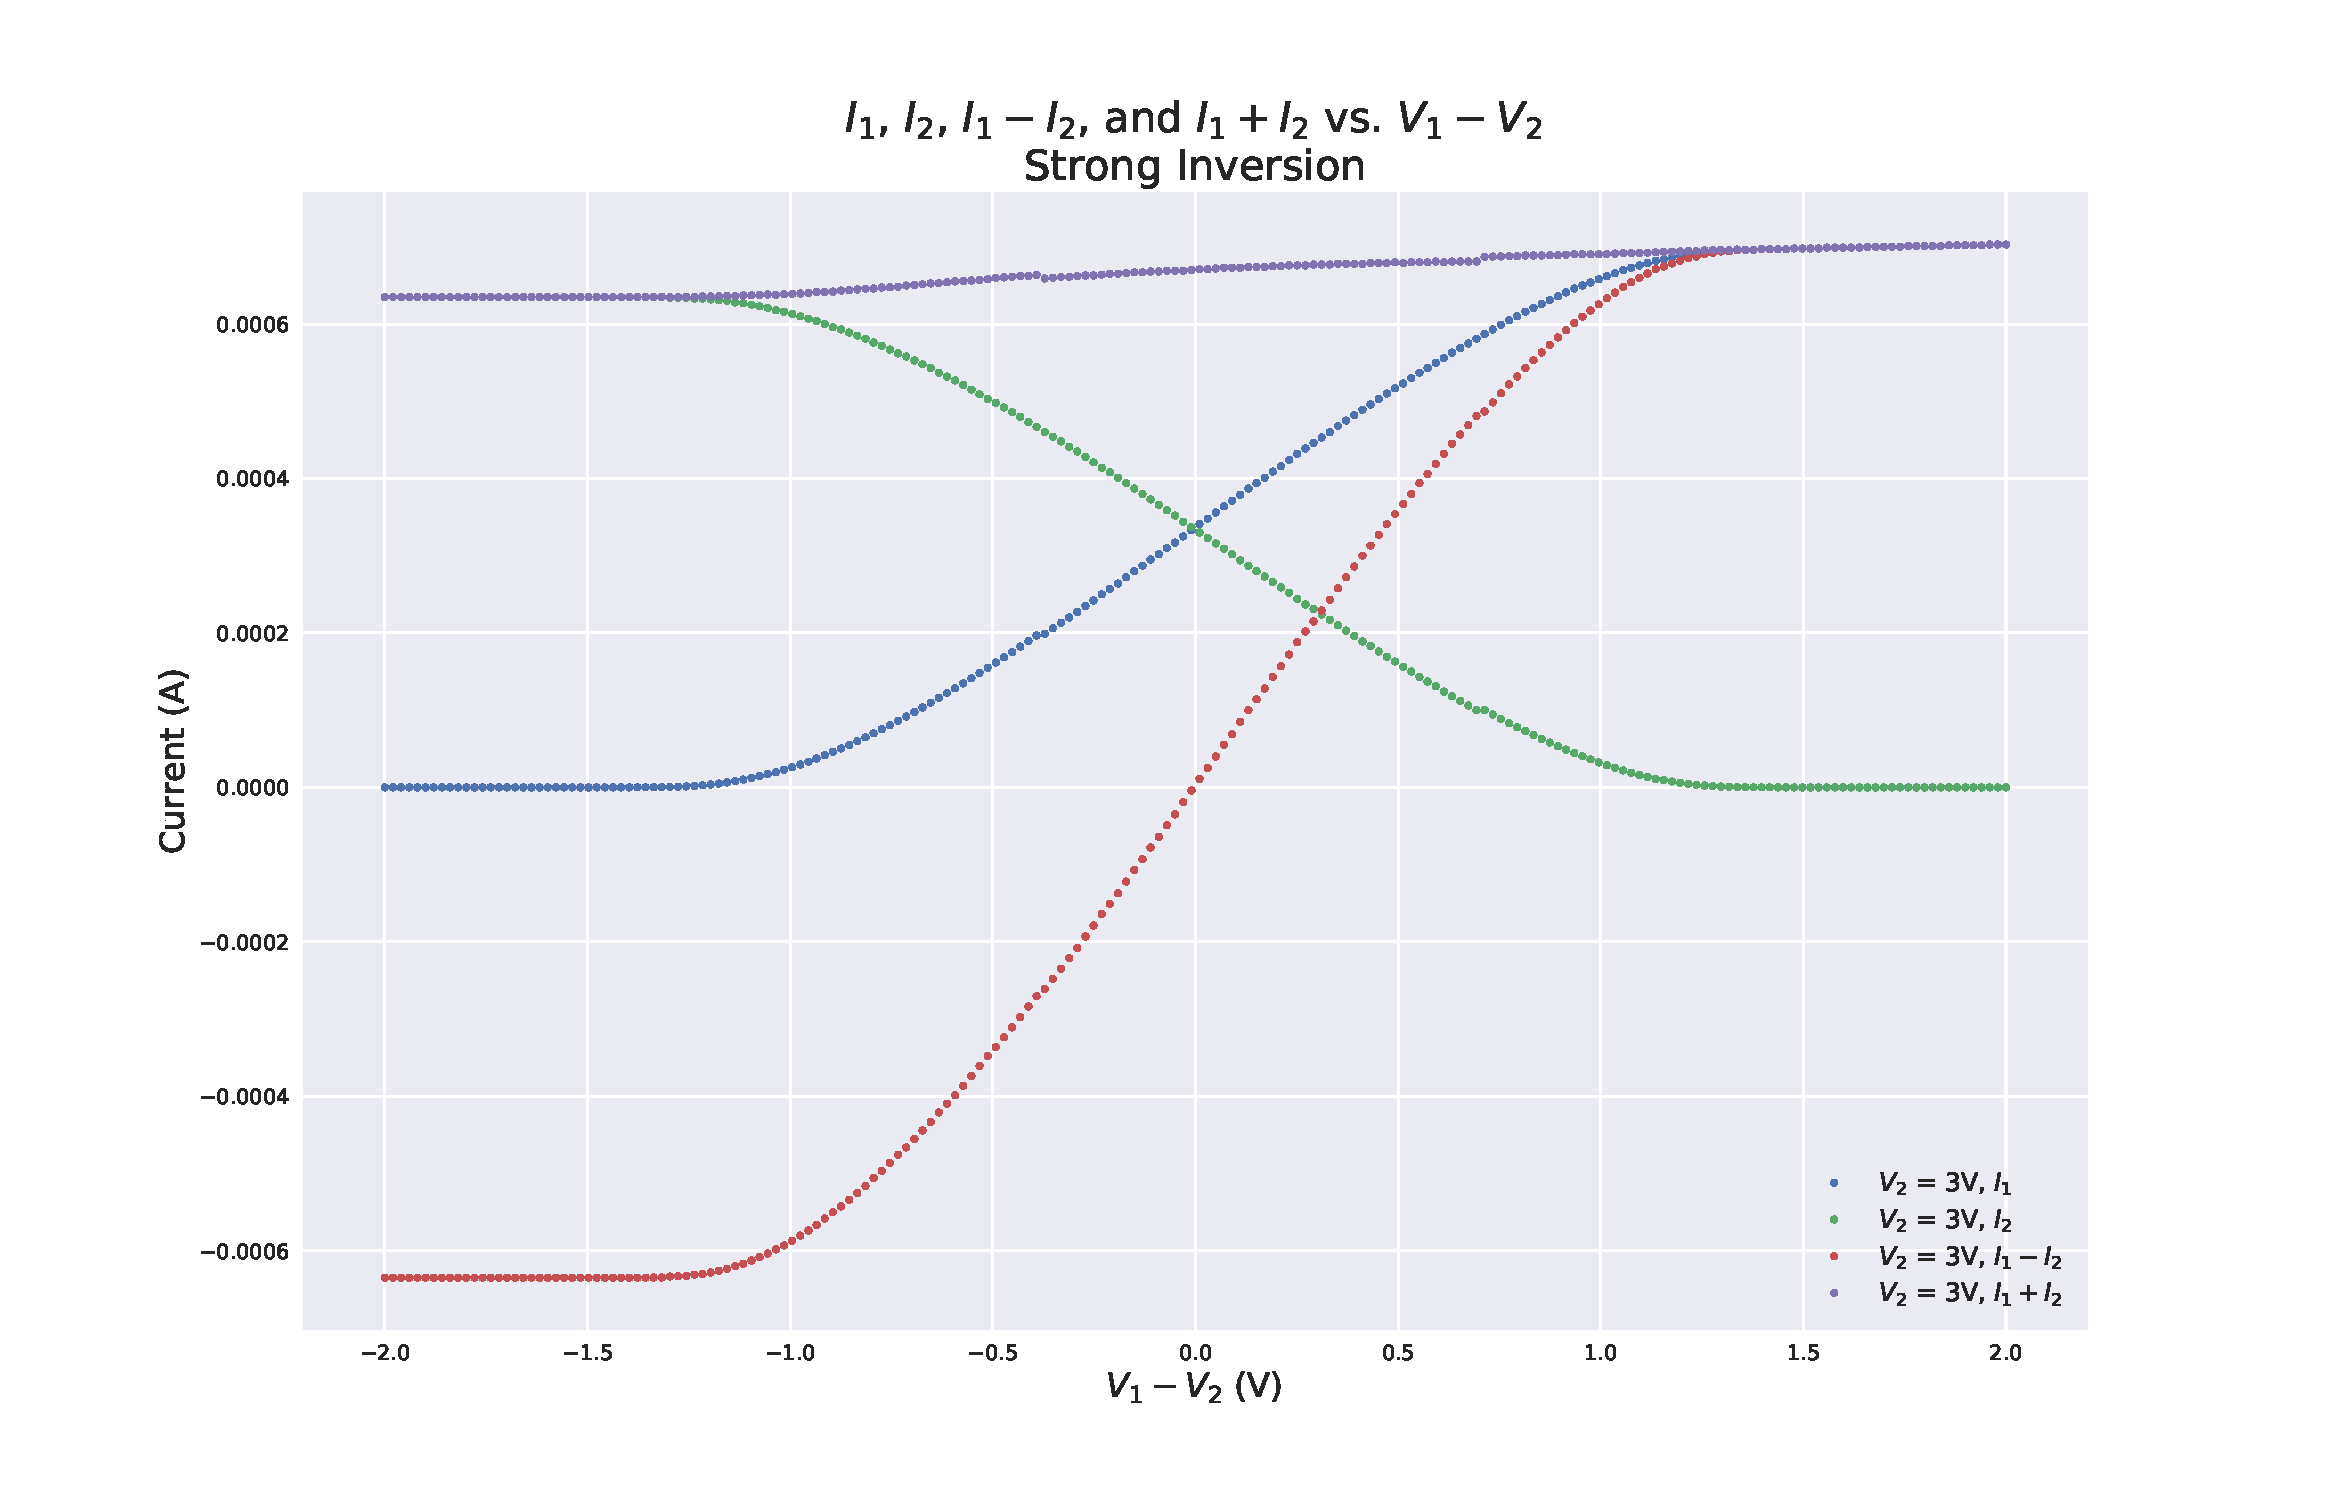
\includegraphics[width=\textwidth]{../strong}
    \caption{Current and Voltage characteristic of pMOS Circuit with a bias voltage that allows for Strong Inversion}
    \label{fig:strong}
\end{figure}

\begin{figure}[h]
    \centering
    \includegraphics[width=\textwidth]{../schematic}
    \caption{Schematic for LTSpice simulation of pMOS Circuit}
    \label{fig:s}
\end{figure}



\end{document}

